\documentclass[11pt]{amsart}
\usepackage[margin=1.1in]{geometry}
\usepackage{amssymb,amsmath,booktabs}
\usepackage{tikz}
\usetikzlibrary{calc}
\usepackage[font=small,labelfont=bf]{caption}
\usepackage[hidelinks]{hyperref}

\colorlet{copper}{orange!75!black}
\colorlet{inkmuted}{black!60}

\newtheorem{theorem}{Theorem}[section]
\newtheorem{proposition}[theorem]{Proposition}
\newtheorem{corollary}[theorem]{Corollary}
\newtheorem{lemma}[theorem]{Lemma}
\theoremstyle{definition}
\newtheorem{definition}[theorem]{Definition}
\newtheorem{hypothesis}[theorem]{Hypothesis}
\newtheorem{observation}[theorem]{Observation}
\theoremstyle{remark}
\newtheorem{remark}[theorem]{Remark}

\newcommand{\Z}{\mathbb{Z}}
\newcommand{\Q}{\mathbb{Q}}
\newcommand{\leg}[2]{\left(\frac{#1}{#2}\right)}

\title{Bogner's strange Calabi-Yau operator carries a $\sqrt2$ twist}
\author{Vamshi Jandhyala}
\address{London, United Kingdom}
\email{vamshi.jandhyala@gmail.com}
\date{Preprint v2, 25 October 2026 (v1: 11 October 2026). Not peer reviewed.}

\begin{document}

\begin{abstract}
Bogner found a fourth order operator of Calabi-Yau type whose holomorphic period is integral, and whose
mirror map and Yukawa coupling are integral in every degree computed, while its instanton numbers are not: $n_p$ has denominator $p^2$ at
every prime $p\ge3$ that has been examined. As Bogner and Reiter found, the operator is the Hadamard
product of $\sum\binom{2n}{n}x^n$ with the symmetric square of a second order operator; we record that this
operator is modular for an index four subgroup of $\mathrm{PSL}_2(\Z)$, and show that the instanton numbers
become integers, for all $d\le110$, when they are read through a Galois twisted multicover formula over
$\Q(\sqrt2)$. The
twist is dictated by the cusp, where the Hauptmodul satisfies $x^4\approx-q_\tau/4$. A twisted form
of a theorem of Beukers and Vlasenko proves the twisted integrality at each prime $p\ge5$ from a
$p$-adic Frobenius structure with a specified first constant. We state the existence of that
structure as a hypothesis, and certify its truncations at $p=5,7,11,13,17$, up to degree $1000$ at
$p=5$; every truncation forces the predicted constant. We also show that rescaling the coordinate
does not help (for algebraic irrational scalings conditional on an all-prime congruence, for rational
ones of bounded height), that the strong structure does not exist at $p=3$, and that two natural
routes to the hypothesis are closed.
\end{abstract}

\maketitle

\section{Introduction}

Let $\theta=x\,\frac{d}{dx}$ and
\[
P=\theta^4-8x(2\theta+1)^2(5\theta^2+5\theta+2)+192x^2(2\theta+1)(3\theta+2)(3\theta+4)(2\theta+3).
\]
This operator appears in Bogner's thesis \cite{Bog12} and is discussed by van Straten
\cite[pp.~28--29]{vS17} and by Almkvist and van Straten \cite[p.~22 of arXiv v1]{AvS}; Bogner and Reiter
obtained it as the entry $8'$ of their table of operators $\mathrm{Sym}^2R\star I_{1/2}$ and noted that it has no
integral instanton numbers \cite[Proposition~3.6 and the table of Section~3]{BR}. It has the holomorphic
solution $y_0=1+16x+576x^2+25600x^3+\cdots$, the mirror map $q=x+40x^2+1984x^3+\cdots$
and the Yukawa coupling
\[
K(q)=1+8q-5632q^3-456064q^4-17708032q^5+\cdots.
\]
The mirror map and the Yukawa coupling have integer coefficients through degree $110$ in our computations;
we know of no proof that they are integral in every degree. (The printed $8q^2$ in \cite{AvS} is a misprint
for $8q$.) Writing
$K(q)=1+\sum_{d\ge1}n_d d^3 q^d/(1-q^d)$ gives $n_1=8$, $n_2=-1$, $n_3=-1880/9$,
$n_5=-3541608/25$, and $n_p$ has denominator $p^2$ for the odd primes tested. Van Straten calls this ``rather
puzzling'': integrality of the period and the mirror map suggests a rank four Calabi-Yau motive, to
which the general integrality arguments should apply. He adds that there may be a different scaling
of the coordinate that repairs the defect.

Table~\ref{tab:first} shows what this note proposes instead. The left column is the usual expansion.
The right column reads the same coupling through a multicover formula twisted by $\sqrt2$
(Section~\ref{sec:twist}), and every entry becomes an integer.

\begin{table}[h]
\centering
\begin{tabular}{rrr}
\toprule
$d$ & untwisted $n_d$ & twisted $n_d$\\
\midrule
$1$ & $8$ & $8$\\
$2$ & $-1$ & $0$\\
$3$ & $-1880/9$ & $-208$\\
$4$ & $-7126$ & $-7126$\\
$5$ & $-3541608/25$ & $-141664$\\
$6$ & $-18136853/9$ & $-2015232$\\
\bottomrule
\end{tabular}
\caption{Instanton numbers of Bogner's operator, untwisted and twisted.}\label{tab:first}
\end{table}

The results are as follows.

\begin{enumerate}
\item (Structure, Section~\ref{sec:structure}; due to Bogner and Reiter \cite{BR}.) $P=I\star\mathrm{Sym}^2 D$, where $I$ is the first order
operator of $\sum\binom{2n}{n}x^n$, $\star$ is the Hadamard product, and $D$ is a second order
operator whose holomorphic solution is
$(1-16x)^{-1/4}\,{}_2F_1\bigl(\tfrac1{12},\tfrac5{12};1;-6912x^4/(1-16x)^3\bigr)$. Equivalently
$j=(16x-1)^3/(4x^4)$.
\item (Scaling obstructions, Section~\ref{sec:scaling}.) Conditional on $K_p\equiv8\pmod p$ for almost all primes, no algebraic irrational rescaling makes the instanton numbers integral at almost all primes. No rational scaling with numerator and denominator at most $3000$ works.
\item (Twisted integrality, Section~\ref{sec:twist}.) With the multicover weights
$w_d(k)=\leg{2}{k}^d 2^{d(k-1)/2}$ for odd $k$ (Section~\ref{sec:twist} treats even $k$) the numbers
defined by
$K_m=\sum_{d\mid m} n_d\,d^3\,w_d(m/d)$ are integers for all $d\le110$.
\item (Explanation, Section~\ref{sec:frobenius}.) The weights come from the Frobenius lift
$q\mapsto c_pq^p$ with $c_p=\leg2p 2^{(p-1)/2}$, which is the lift the cusp of $D$ dictates.
A twisted form of a theorem of Beukers and Vlasenko \cite{BV} turns a Frobenius structure with first
constant $\log_p(c_p)/p$ into twisted integrality at $p\ge5$. Finite truncations of such a
structure exist at $p=5,7,11,13,17$ and force that constant.
\item (Approaches, Section~\ref{sec:approaches}.) Models of the period, and proofs or
computations that close two routes to the remaining hypothesis.
\end{enumerate}

All computations use exact rational arithmetic. The scripts that produce each number are listed in
Section~\ref{sec:data}.

\section{Structure of the operator}\label{sec:structure}

\begin{proposition}\label{prop:structure}
Let
\begin{align*}
D&=\theta^2-4x(10\theta^2+5\theta+1)+48x^2(3\theta+1)(3\theta+2),\\
L&=\theta^3-4x(2\theta+1)(5\theta^2+5\theta+2)+48x^2(\theta+1)(3\theta+2)(3\theta+4).
\end{align*}
Then $L=\mathrm{Sym}^2 D$ and $P=I\star L$ \cite[Proposition~3.6, entry $8'$]{BR}. In particular the holomorphic solution of $P$ is
$y_0=\sum_n\binom{2n}{n}u_nx^n$ where $\sum_n u_nx^n=f^2$ and $f$ is the holomorphic solution of $D$.
\end{proposition}

\begin{proof}
We include the short verification. The symmetric square of a second order operator is computed by the recursion in
\cite[Lemma~4.2.4]{Bog12}; comparing normalised coefficients with those of $L$ gives equality as
rational functions (checked symbolically). If $(n+1)^3u_{n+1}=R_1(n)u_n-R_2(n)u_{n-1}$ with
$R_1=4(2n+1)(5n^2+5n+2)$ and $R_2=48n(9n^2-1)$, then $v_n=\binom{2n}{n}u_n$ satisfies
$(n+1)^4v_{n+1}=2(2n+1)R_1(n)v_n-4(4n^2-1)(R_2(n)/n)v_{n-1}$, which is the recurrence of $P$.
\end{proof}

The operator $D$ has singular points $0$, the complex conjugate pair
$x_\pm=(5\pm i\sqrt2)/108$ and $\infty$, with local exponents $\{0,0\}$, $\{0,\tfrac12\}$ and
$\{\tfrac13,\tfrac23\}$. This is the signature of a genus zero group with one cusp, two elliptic
points of order two and one of order three.

\begin{proposition}\label{prop:modular}
The holomorphic solution of $D$ is
\[
f(x)=(1-16x)^{-1/4}\;{}_2F_1\!\left(\tfrac1{12},\tfrac5{12};1;\,\frac{-6912x^4}{(1-16x)^3}\right).
\]
Equivalently, $f$ is the pullback of $E_4^{1/4}={}_2F_1(\tfrac1{12},\tfrac5{12};1;1728/j)$ along
\[
j=\frac{(16x-1)^3}{4x^4},\qquad j-1728=-\frac{(1-4x)^2(432x^2-40x+1)}{4x^4},
\]
a degree four map ramified as $(4)$ over $\infty$, $(3,1)$ over $0$ and $(2,1,1)$ over $1728$.
Hence $x$ is a Hauptmodul for an index four subgroup of $\mathrm{PSL}_2(\Z)$ with one cusp, of width four.
\end{proposition}

\begin{proof}
Write $g=(1-16x)^{-1/4}F(z(x))$ with $z(x)=-6912x^4/(1-16x)^3$ and $F$ any solution of the Gauss
equation with parameters $(\tfrac1{12},\tfrac5{12};1)$. Eliminating $F''$ with the Gauss equation,
$D(g)$ simplifies to zero (checked symbolically). Since $D$ has exponents $0,0$ at the origin, the
holomorphic solution with value $1$ is unique. The factorisation of $j-1728$ is direct, and a
branched cover of the $j$-line with ramification indices dividing $\infty,3,2$ over
$\infty,0,1728$ corresponds to a finite index subgroup.
\end{proof}

Near the cusp, $1/j=-4x^4+O(x^5)$, so the Tate parameter satisfies
\begin{equation}\label{eq:cusp}
q_\tau=-4x^4\bigl(1+O(x)\bigr).
\end{equation}
The Frobenius compatible coordinate at the cusp is therefore $(-4)^{1/4}x=(1+i)x$ up to a fourth
root of unity. This constant drives everything in Sections~\ref{sec:twist} and~\ref{sec:frobenius}.
Figure~\ref{fig:cover} shows the cover and where the constant comes from.

\begin{figure}[ht]
\centering
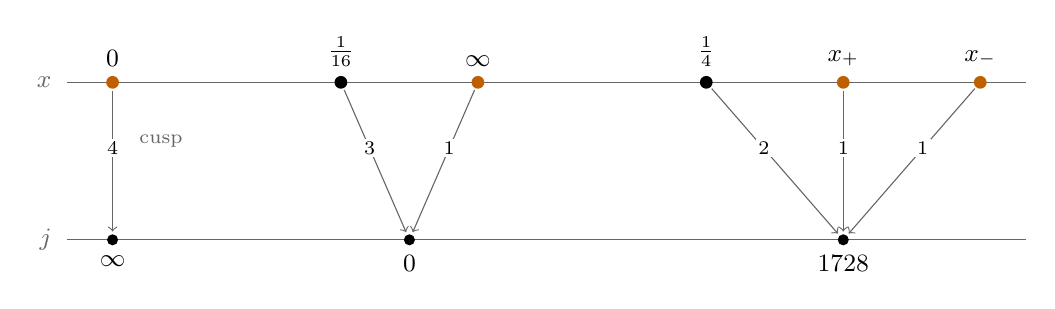
\begin{tikzpicture}[x=1.45cm,y=1cm,font=\small]
  % x-line
  \draw[inkmuted,thin] (-0.4,2) -- (8.0,2);
  \node[anchor=east,inkmuted] at (-0.45,2) {$x$};
  % j-line
  \draw[inkmuted,thin] (-0.4,0) -- (8.0,0);
  \node[anchor=east,inkmuted] at (-0.45,0) {$j$};
  % images
  \foreach \u/\lab in {0/{\infty},2.6/{0},6.4/{1728}}
    {\fill (\u,0) circle (2pt); \node[below] at (\u,-0.08) {$\lab$};}
  % preimages: position, label, image, index, singular?
  \foreach \x/\lab/\u/\e/\col in {0/{0}/0/4/copper, 2.0/{\tfrac1{16}}/2.6/3/black, 3.2/{\infty}/2.6/1/copper,
                                   5.2/{\tfrac14}/6.4/2/black, 6.4/{x_+}/6.4/1/copper, 7.6/{x_-}/6.4/1/copper}
    {\draw[inkmuted,->,shorten <=3pt,shorten >=3pt] (\x,2) -- (\u,0);
     \fill[\col] (\x,2) circle (2.3pt);
     \node[above] at (\x,2.08) {$\lab$};
     \node[fill=white,inner sep=1pt,font=\scriptsize] at ($(\x,2)!0.42!(\u,0)$) {$\e$};}
  \node[anchor=west,font=\scriptsize,inkmuted] at (0.15,1.25) {cusp};
\end{tikzpicture}

\caption{The degree four map $j=(16x-1)^3/(4x^4)$ from the $x$-line to the $j$-line, with the
ramification of Proposition~\ref{prop:modular}. The cusp $x=0$ lies over $j=\infty$ with index
$4$, and there $1/j=-4x^4+O(x^5)$: a fourth root of $-4$, hence $\sqrt2$, enters the coordinate
compatible with $q_\tau\mapsto q_\tau^p$. Singular points of $D$ are in copper.}
\label{fig:cover}
\end{figure}

\begin{remark}
$D$ is, up to the algebraic gauge factor $(432x^2-40x+1)^{1/4}$, the Picard-Fuchs operator of the
rational elliptic surface
\[
Y^2=4X^3-3(1-16x)(432x^2-40x+1)\,X-(1-4x)(432x^2-40x+1)^2,
\]
whose $j$-invariant is $(16x-1)^3/(4x^4)$ and whose discriminant is
$-186624\,x^4(432x^2-40x+1)^3$. Its singular fibres are $I_4$ at $0$, $III$ at $x_\pm$ and $II$ at
$\infty$.
\end{remark}

\begin{corollary}
Via Clausen's formula,
\[
u_n=\sum_{m=0}^{\lfloor n/4\rfloor}(-1)^m\,4^{\,n-3m}\,\frac{(2n-2m)!}{m!^3\,(n-m)!\,(n-4m)!},
\]
and $y_0=\sum\binom{2n}{n}u_nx^n$. In particular $u_n$ and $y_0$ have integer coefficients: the factorial ratio is a multinomial coefficient and $n-3m\ge0$ throughout the sum. The sequence $u_n=1,8,96,1280,17440,\dots$ is not in the OEIS
(searched 27 September 2026). The formula agrees with the recurrence of $L$ for $n\le 120$.
\end{corollary}

\begin{proposition}\label{prop:ct}
Let $h(Y)=Y+2+Y^{-1}$. Then, as formal power series in $t$,
\begin{align*}
\sum_n u_nt^n&=\mathrm{CT}_{a,b,Y}\,\frac{1}{1-4t\,h(Y)(1+a+b)+\tfrac{t^2}{4}\,h(Y)/(ab)},\\
y_0&=\mathrm{CT}_{a,b,Y,Z}\,\frac{1}{1-4t\,h(Y)h(Z)(1+a+b)+\tfrac{t^2}{4}\,h(Y)h(Z)^2/(ab)} .
\end{align*}
\end{proposition}

\begin{proof}
Expand $[t^n](1-tA+t^2B)^{-1}=\sum_k(-1)^k\binom{n-k}{k}A^{n-2k}B^k$. With $A=4h(Y)(1+a+b)$ and
$B=h(Y)/(4ab)$, the constant term in $a,b$ of $(1+a+b)^{n-2k}(ab)^{-k}$ is
$(n-2k)!/(k!^2(n-4k)!)$ and $\mathrm{CT}_Y\,h(Y)^{n-k}=\binom{2n-2k}{n-k}$. Collecting factors gives
the closed form of the corollary. The second identity follows from $\mathrm{CT}_Z\,h(Z)^n=\binom{2n}{n}$.
\end{proof}

\begin{corollary}\label{cor:doublecover}
There is also a three-variable double-cover period representation
\[
y_0(t)=\mathrm{CT}_{a,b,Z}\left(1-16t\,h(Z)(1+a+b)
                  +\frac{t^2h(Z)^2}{ab}\right)^{-1/2}.
\]
\end{corollary}
\begin{proof}
For a formal series $C$ of positive $t$-adic order,
$\mathrm{CT}_Y(1-C h(Y))^{-1}=\sum_{r\ge0}\binom{2r}{r}C^r=(1-4C)^{-1/2}$.
Use $C=4t h(Z)(1+a+b)-t^2h(Z)^2/(4ab)$ in Proposition~\ref{prop:ct}.
\end{proof}

\section{Obstructions to rescaling}\label{sec:scaling}

The Yukawa coupling is an invariant of $P$ up to $q\mapsto cq$ \cite{vS17}. Rescaling replaces
$K_m$ by $c^mK_m$.

\begin{proposition}\label{prop:irrational}
Let $c$ be a nonzero algebraic number. Assume $K_p\equiv 8\pmod p$ for all but finitely many primes $p$
(it holds for every odd $p\le109$, and would follow from \eqref{eq:Cp} at all odd primes). If the instanton numbers of
$K(cq)$ are integral at all but finitely many primes, then $c\in\Q$.
\end{proposition}

\begin{proof}
Let $F$ be the Galois closure of $\Q(c)$. For a prime $\mathfrak p$ of $F$ above $p$, unramified,
with $c$ a $\mathfrak p$-unit and $p\nmid 2$, integrality of $n_p(c)=(c^pK_p-8c)/p^3$ gives
$c^pK_p\equiv 8c\pmod{\mathfrak p}$. Since $K_p\equiv 8\pmod p$, this gives
$c^p\equiv c\pmod{\mathfrak p}$, that is
$\mathrm{Frob}_{\mathfrak p}(c)\equiv c\pmod{\mathfrak p}$. For each $\sigma\in\mathrm{Gal}(F/\Q)$ with
$\sigma(c)\ne c$ the nonzero number $\sigma(c)-c$ is divisible by only finitely many primes, while by
Chebotarev $\sigma=\mathrm{Frob}_{\mathfrak p}$ for infinitely many $\mathfrak p$. Hence $\sigma(c)=c$
for all $\sigma$.
\end{proof}

\begin{proposition}\label{prop:rational}
For every $c=\pm a/b$ with $1\le a,b\le 3000$ there is a prime $p\le 79$, $p\nmid ab$, with
$c^{p-1}K_p\not\equiv 8\pmod{p^2}$. In particular some instanton number of $K(cq)$ fails to be
$p$-integral.
\end{proposition}

This is a finite computation over Fermat quotients. The same search, run on data planted with
$c=17/5$, returns exactly that value.

\section{The twisted multicover formula}\label{sec:twist}

For $d,k\ge1$ put
\[
w_d(k)=\begin{cases}
\leg{2}{k}^d\,2^{d(k-1)/2} & k \text{ odd},\\
2^{d(k-1)/2} & k \text{ even},\ d \text{ even},\\
0 & k \text{ even},\ d \text{ odd},
\end{cases}
\]
with the Jacobi symbol $\leg2k$, and define $n_d$ recursively by
$K_m=\sum_{d\mid m}n_d\,d^3\,w_d(m/d)$. In words, the coefficient $K_m$ collects, for each $d\mid m$,
the degree $d$ number $n_d$ counted $k=m/d$ times over; the classical formula gives each $k$-fold
cover weight $1$, and the twisted one gives it weight $w_d(k)$.

\begin{remark}
With $Q=\sqrt2\,q$ and $\nu_d=n_d\,2^{-d/2}$ this reads
\[
K(Q/\sqrt2)=1+\sum_d d^3\sum_k \mathrm{Frob}_k(\nu_d)\,Q^{dk},
\]
where, for odd $k$, $\mathrm{Frob}_k$ acts on $\Q(\sqrt2)$ by $\sqrt2\mapsto\leg2k\sqrt2$. For even $k$ the displayed symbol denotes instead the projection $\nu\mapsto(\nu+\bar\nu)/2$ to $\Q$. This even-multiplier convention is part of our definition, not a Frobenius automorphism at the ramified prime $2$. The formula is Galois equivariant for odd multipliers.
\end{remark}

\begin{observation}\label{obs:integral}
The numbers $n_d$ are integers for all $d\le 110$. The first are
\[
8,\ 0,\ -208,\ -7126,\ -141664,\ -2015232,\ -3250624,\ 1056216756,\ 46257581056,\ \dots
\]
With the untwisted weights $w\equiv1$, $76$ of the first $80$ are not integers.
\end{observation}

The weights are rigid. Replacing $\sqrt2$ by $\sqrt3$, dropping the sign, using $\leg{-1}{k}$, or
using $\leg2k$ in place of $\leg2k^d$ each produces non-integral values within $d\le 80$, and so does
altering $K_{45}$ by $45^2$.

At a single odd prime the formula is equivalent to a twisted Dwork congruence. Put
\[
c_p=\leg2p\,2^{(p-1)/2}\equiv1\pmod p .
\]

\begin{observation}\label{obs:congruence}
For every odd prime $p$ and every $n\le110$ divisible by $p$,
\begin{equation}\label{eq:Cp}
K_n\equiv c_p^{\,n/p}\,K_{n/p}\pmod{p^{3v_p(n)}} .
\end{equation}
There are $135$ such pairs $(p,n)$, including $p=3,n=81$ modulo $3^{12}$, and all hold. With
$c_p=1$ only $16$ hold. With $c_p=2^{(p-1)/2}$ (no sign), $82$ hold.
\end{observation}

For comparison, Table~\ref{tab:controls} lists Hadamard products $I\star L'$ for classical third
order operators $L'$, each the symmetric square of a modular operator with a cusp of width one. Their
untwisted instanton numbers fail to be integral only at a few primes, as expected from
$N$-integrality. The operator $P$ fails at every prime, which is a different phenomenon.

\begin{table}[h]
\centering
\begin{tabular}{lc}
\toprule
$L'$ & primes in denominators of $n_d$, $d\le 20$\\
\midrule
Ap\'ery $\zeta(3)$ & $2,3$\\
Domb & $3$\\
Almkvist-Zudilin & none\\
Cooper $s_7$ & $2,7$\\
Cooper $s_{10}$ & $5$\\
$L$ (this paper) & every prime $p\le19$\\
\bottomrule
\end{tabular}
\caption{Untwisted instanton numbers of $I\star L'$.}\label{tab:controls}
\end{table}

\section{Frobenius structures}\label{sec:frobenius}

We use the framework of Beukers and Vlasenko \cite{BV}. Let $p$ be an odd prime and $\sigma$ a
Frobenius lift on $\Z_p[[x]]$. A $p$-adic Frobenius structure for $P$ is an operator
$A=\sum_{i=0}^3A_i(x)\theta^i$ with $A_i\in\Z_p[[x]]$ and $A_0(0)=1$ such that $A(y(x^\sigma))$ is
a solution whenever $y$ is \cite[Def.~1.1]{BV}. For the lift $x^\sigma=x^p$ the Frobenius basis
$y_0,\dots,y_3$ satisfies $A(y_i^\sigma)=p^i\sum_{j\le i}\alpha_jy_{i-j}$ \cite[Remark~1.2]{BV}.
Beukers and Vlasenko prove that if $P$ is self dual and $\alpha_1=0$, then the untwisted
instanton numbers are $p$-integral \cite[Thm.~1.7]{BV}. The operator $P$ is self adjoint, since each
coefficient $Q_j(\theta)$ of $x^j$ satisfies $Q_j(-\theta-j)=Q_j(\theta)$.

\begin{lemma}[Integral change of lift in rank four]\label{lem:transport}
Let $p\ge5$. Suppose $z_0,\ldots,z_3$ solve a monic fourth order equation in
$\Z_p[[q]][\theta_q]$. Let $s_0(q)$ and $s_1(q)=c q^p$ be Frobenius lifts with
$c\in1+p\Z_p$ and $s_0/s_1\in1+p\Z_p[[q]]$.
There is $T\in\Z_p[[q]][\theta_q]$ such that
$T(z_i(s_1))=z_i(s_0)$ for every $i$.
\end{lemma}
\begin{proof}
Write $h=\log(s_0/s_1)\in p\Z_p[[q]]$. Reduce each power $\theta_z^k$ modulo
the monic source equation as $\sum_{i=0}^3r_{ki}(z)\theta_z^i$, with
$r_{ki}\in\Z_p[[z]]$. For $k<4$ this is just $r_{ki}=\delta_{ki}$.
Taylor's formula gives, on solutions,
\[
z_i(s_0)=\sum_{k\ge0}\frac{h^k}{k!}(\theta_z^k z_i)(s_1)
=\sum_{j=0}^3b_j(q)(\theta_z^j z_i)(s_1),\qquad
b_j=\sum_{k\ge0}\frac{h^k}{k!}r_{kj}(s_1).
\]
These sums converge $p$-adically. For $k\ge4$ and $p\ge5$,
$k-v_p(k!)\ge3$, while the $k<4$ terms give $b_j\in p^j\Z_p[[q]]$ directly.
Consequently every $b_j$ belongs to $p^j\Z_p[[q]]$.
Since $(\theta_z^jz_i)(s_1)=p^{-j}\theta_q^j(z_i(s_1))$, take
$T=\sum_jp^{-j}b_j\theta_q^j$.
This proof explains why an unreduced Taylor series with integral coefficients
cannot simply be asserted, and why $p=3$ needs a separate argument.
\end{proof}

\begin{theorem}\label{thm:twisted}
Let $p\ge5$. Suppose $P$ has a $p$-adic Frobenius structure for the lift $x\mapsto x^p$
with $\alpha_1=\frac1p\log_p c_p$. Then $K\in\Z_p[[q]]$ and \eqref{eq:Cp} holds for all
$n$ divisible by $p$. The twisted numbers $n_d$ are $p$-integral for every $d$.
\end{theorem}

\begin{proof}
Theorem~1.4 and Lemma~2.3 of \cite{BV} give $q\in x+x^2\Z_p[[x]]$ and
$y_0\in1+x\Z_p[[x]]$. Dividing solutions by $y_0$ and changing to $q$ therefore
preserves integrality of the monic equation and of the Frobenius operator.
Let $z_i=y_i/y_0$, $\Lambda=\log q$, and $\ell=p\alpha_1=\log_p c_p$.
The original lift becomes $s_0(q)=q(x(q)^p)$, with $s_0/q^p\in1+p\Z_p[[q]]$.
Lemma~\ref{lem:transport} transports its operator to the lift
$s_1(q)=c_pq^p$, preserving the action
\[
A(z_i(s_1))=p^i\sum_{j\le i}\alpha_jz_{i-j}.
\]
The transported operator has integral coefficients; composition followed by
reduction modulo the pulled-back monic equation keeps them integral.

Put $a=\ell/(p-1)\in p\Z_p$, $M=\Lambda+a$, and
$\widetilde z_i=\sum_{j=0}^i a^{i-j}z_j/(i-j)!$.
Their first four expressions are
\[
1,\quad M,\quad \tfrac12M^2+V_2,\quad
\tfrac16M^3+M V_2+V_3.
\]
Since $M(s_1)=pM$, the action on this basis has constants
$\beta_i=[u^i](\sum_j\alpha_j u^j)e^{-\alpha_1u}$.
In particular $\beta_1=0$,
$\beta_2=\alpha_2-\alpha_1^2/2$ and
$\beta_3=\alpha_3-\alpha_1\alpha_2+\alpha_1^3/3$, all in $\Z_p$.
From $A(1)=1$ and $A(M)=M$ we obtain $A=1+B\theta_q^2$ with
$B\in\Z_p[[q]][\theta_q]$.

In the following, a superscript $\sigma$ means composition with $s_1$.
Applying $A$ to $\widetilde z_2^\sigma$ gives
\begin{equation}\label{eq:V2}
p^{-2}V_2^\sigma-V_2=\beta_2-BK^\sigma,\qquad K=1+\theta_q^2V_2.
\end{equation}
Taking two derivatives yields $(1+\theta_q^2\circ B)K^\sigma=K$.
The contraction argument of \cite[Lemma~2.3]{BV} also applies to $s_1=c_pq^p$,
since it increases $q$-adic order by $p$. Hence $K\in\Z_p[[q]]$.

Self-duality gives $2V_2+\theta_qV_3=0$. It follows that
$\theta_q^2\widetilde z_3^\sigma=p^3 M K^\sigma$.
Apply $A$ to $\widetilde z_3^\sigma$ and subtract $M$ times \eqref{eq:V2}; this gives
\[
\psi:=p^{-3}V_3^\sigma-V_3
=\beta_3-[B,M]K^\sigma\in\Z_p[[q]].
\]
Here $[B,M]$ is integral: if $B=\sum b_j\theta_q^j$ then
$[B,M]=\sum j b_j\theta_q^{j-1}$.
Taking three derivatives and using self-duality once more gives
\[
K(c_pq^p)-K(q)=-\tfrac12\theta_q^3\psi.
\]
At degree $n$ divisible by $p$, its left side is
$c_p^{n/p}K_{n/p}-K_n$, and its right side belongs to $n^3\Z_p$.
This proves \eqref{eq:Cp}; the last assertion follows from the next lemma.
\end{proof}

\begin{lemma}[Twisted multicover integrality]\label{lem:multicover}
Fix an odd prime $p$ and suppose $K_m\in\Z_p$ for every $m$.
For the weights of Section~\ref{sec:twist}, the congruences \eqref{eq:Cp} for all $p\mid m$
are equivalent to $n_d\in\Z_p$ for every $d$.
\end{lemma}
\begin{proof}
For every $d,k\ge1$ one has
\begin{equation}\label{eq:weightcompatibility}
w_d(pk)=c_p^{dk}w_d(k).
\end{equation}
For odd $k$ use multiplicativity of the Jacobi symbol and $dk\equiv d\pmod2$.
For even $k$ and odd $d$ both sides vanish; for even $k$ and even $d$ the
sign is $1$ and the equality follows by subtracting the exponents of $2$.
Also $w_d(1)=1$ and all weights are integers.

Write $m=p^r u$ with $p\nmid u$ and $r\ge1$.
Subtract $c_p^{m/p}K_{m/p}$ from $K_m$. Equation~\eqref{eq:weightcompatibility}
cancels precisely the terms with $d\mid m/p$, leaving
\[
K_m-c_p^{m/p}K_{m/p}
=\sum_{\substack{d\mid m\\v_p(d)=r}}n_d d^3 w_d(m/d).
\]
If all $n_d$ are $p$-integral, this belongs to $p^{3r}\Z_p$.
Conversely, induct on $m$. When $p\nmid m$, the defining recursion and
$K_m\in\Z_p$ prove integrality of $n_m$ because $m^3$ is a unit.
When $p\mid m$, all terms in the last sum with $d<m$ lie in $p^{3r}\Z_p$ by
induction. The congruence then puts its remaining term $m^3n_m$ in
$p^{3r}\Z_p$, so $n_m\in\Z_p$ as well.
\end{proof}

\begin{remark}
Theorem~\ref{thm:twisted} proves no assertion at $p=2,3$. In particular, a proof
of Hypothesis~\ref{hyp:F} would establish integrality away from $2,3$, not
integer-valuedness without further work at these two primes.
\end{remark}

The value of $\alpha_1$ in the theorem is the one the cusp predicts.

\begin{proposition}\label{prop:alpha}
For every odd prime $p$, $c_p\equiv1\pmod p$ and $c_p^4=(-4)^{p-1}$. Consequently the lift of the
$x$-line that corresponds to $q_\tau\mapsto q_\tau^p$ under \eqref{eq:cusp} has the form
$x\mapsto c_p\,x^p(1+O(x))$.
\end{proposition}

\begin{proof}
By Euler's criterion $2^{(p-1)/2}\equiv\leg2p\pmod p$, so $c_p\equiv1$. Also
$c_p^4=2^{2(p-1)}=4^{p-1}=(-4)^{p-1}$. If $x^\sigma=c\,x^p(1+O(x))$ and $q_\tau(x^\sigma)=q_\tau(x)^p$,
comparing leading terms in \eqref{eq:cusp} gives $-4c^4=(-4)^p$, so $c^4=(-4)^{p-1}$, and $c\equiv1$
singles out $c=c_p$ among the fourth roots.
\end{proof}

This explains where the value of $\alpha_1$ comes from. Heuristically, $D$ inherits a Frobenius
structure from Dwork's theory of the Gauss equation, pulled back along $z(x)$ (the gauge factor
$(1-16x)^{-1/4}$ contributes a unit of $1+p\Z_p[[x]]$), and the canonical lift of the Tate curve
$q_\tau\mapsto q_\tau^p$ then gives $\alpha_1=\frac1p\log_pc_p$. We have not made this chain
rigorous. Integrality does not determine $\alpha_1$ for $L$ (Observation~\ref{obs:transfer}), so
the value cannot be read off from $L$ alone, and the natural hypothesis concerns $P$ directly.

\begin{proposition}[An obstruction at the prime $3$]\label{prop:prime3-obstruction}
The operator $P$ has no BV-strong Frobenius structure for the lift
$x\mapsto x^3$ with coefficients in $\Z_3[[x]]$ and $A_0(0)=1$.
\end{proposition}
\begin{proof}
Write $A=\sum_{i=0}^3\sum_{N\ge0} A_{i,N}x^N\theta^i$, and let
$\alpha_1,\alpha_2,\alpha_3$ be its Frobenius constants. Comparing the
coefficient of $x^0$ in the Frobenius identity gives
$A_{i,0}=\alpha_i$, so all three constants must lie in $\Z_3$.
The coefficient recurrence for that identity, computed directly from $P$,
gives
\[
A_{3,3}=-\frac{114512}{9}+\frac{766216}{9}\alpha_1
       +90440\alpha_2+25456\alpha_3,
\]
and
\begin{align*}
A_{2,9}={}&\frac{64339413849976508288}{55125}
 -\frac{539829813570751232}{1575}\alpha_1\\
 &-241119247830016\alpha_2-1373373545472\alpha_3.
\end{align*}
Their integrality would imply, respectively,
\[
0\equiv 9A_{3,3}\equiv4+\alpha_1\pmod9,
\qquad
0\equiv 9A_{2,9}\equiv7+7\alpha_1\pmod9.
\]
Thus $\alpha_1\equiv5\pmod9$ and $\alpha_1\equiv8\pmod9$, a contradiction.
These are exact rational coefficient identities; the standalone calculation
\texttt{prime3\_obstruction.py} verifies them without the Hadamard model or
the affine-lattice solver.
\end{proof}

This obstruction concerns the specified strong Frobenius structure and lift.
It does not contradict the twisted Yukawa congruences at $3$, which hold in
the tested range, and does not rule out a different argument for them.

\begin{hypothesis}\label{hyp:F}
For every prime $p\ge5$, $P$ has a $p$-adic Frobenius structure in the sense of \cite[Def.~1.1]{BV}
for the lift $x\mapsto x^p$, with $\alpha_1=\frac1p\log_pc_p$.
\end{hypothesis}

\begin{corollary}
Under Hypothesis~\ref{hyp:F}, the congruences \eqref{eq:Cp} hold for every prime $p\ge5$ and all $n$.
\end{corollary}

The hypothesis can be tested directly. Write the Frobenius basis as
$Y(x,\varepsilon)=\sum_nA_n(\varepsilon)x^{n+\varepsilon}$ and $A=\sum_iA_i(x)\theta^i$ with
$A_i=\sum_rA_{i,r}x^r$. By \cite[Remark~1.2]{BV} the defining property is
$A(Y(x^p,\varepsilon))=\alpha(p\varepsilon)\,Y(x,p\varepsilon)$ modulo $\varepsilon^4$, with
$\alpha(\varepsilon)=\sum_j\alpha_j\varepsilon^j$ and $\alpha_0=1$. Comparing coefficients of
$x^{N+p\varepsilon}$ gives
\[
\sum_{\substack{0\le r\le N\\ r\equiv N\ (p)}}\ \sum_{i=0}^3 A_{i,r}\,(N-r+p\varepsilon)^i\,
A_{(N-r)/p}(\varepsilon)=\alpha(p\varepsilon)\,A_N(p\varepsilon)\pmod{\varepsilon^4}.
\]
The term $r=N$ is $\sum_iA_{i,N}(p\varepsilon)^i$, so the system is triangular: each $A_{i,N}$ is an
affine function of $\alpha_1,\alpha_2,\alpha_3$ with rational coefficients. The strong integrality
$A_{i,N}\in\Z_p$ then becomes a condition on the $\alpha_j$.

\begin{observation}\label{obs:frob}
For $P$ there exist $\alpha_1,\alpha_2,\alpha_3\in\Z_p$ for which every $A_{i,N}$ with $N\le R$
lies in $\Z_p$, and every such choice has the predicted first constant:
\begin{center}
\begin{tabular}{cccc}
\toprule
$p$ & $R$ & $\alpha_1$ forced to & $\frac1p\log_pc_p$\\
\midrule
$5$ & $30$ & $509 \bmod 5^4$ & $509 \bmod 5^4$\\
$7$ & $40$ & $22 \bmod 7^2$ & $22 \bmod 7^2$\\
$11$ & $60$ & $8 \bmod 11^2$ & $8 \bmod 11^2$\\
$13$ & $70$ & $86 \bmod 13^2$ & $86 \bmod 13^2$\\
$17$ & $80$ & $270 \bmod 17^2$ & $270 \bmod 17^2$\\
$5$ & $500$ & $13634 \bmod 5^6$ & $13634 \bmod 5^6$\\
$7$ & $500$ & $47748 \bmod 7^6$ & $47748 \bmod 7^6$\\
$5$ & $650$ & $310509 \bmod 5^8$ & $310509 \bmod 5^8$\\
$5$ & $1000$ & $310509 \bmod 5^8$ & $310509 \bmod 5^8$\\
$7$ & $700$ & $47748 \bmod 7^6$ & $47748 \bmod 7^6$\\
$11$ & $500$ & $4848 \bmod 11^4$ & $4848 \bmod 11^4$\\
$13$ & $500$ & $4142 \bmod 13^4$ & $4142 \bmod 13^4$\\
\bottomrule
\end{tabular}
\end{center}
The same computation for $I\star L'$ with $L'$ the Ap\'ery, Almkvist-Zudilin and Domb operators
forces $\alpha_1\equiv0$ (modulo $5^2$, and modulo $7^2$ for the first two), as the untwisted theory
predicts. For $L$ itself the condition leaves $\alpha_1$ free in this range
(Observation~\ref{obs:transfer}).
\end{observation}

The rows are certified by an exact affine-lattice computation, rather than
by stopping a digit search at a specified precision. For each row condition
$c+v\alpha\in\Z_p$, intersect the current lattice $\alpha=b+B\Z_p^3$ with that
condition by solving one linear congruence. Direct substitution verifies that the
resulting base and every basis column satisfy every coefficient condition.
In all rows above the entire solution set is
$\alpha_1=r+p^s\Z_p$, $\alpha_2,\alpha_3\in\Z_p$, with $r,s$ as tabulated.
Thus the exact predicted $p$-adic value of $\alpha_1$ is admissible in every
truncation checked.

There is a precise passage from finite to infinite structures, but it requires
truncations of every degree, not just arbitrarily many digits at one degree.
\begin{proposition}\label{prop:compactness}
Fix $p\ge5$ and $\alpha_1=\log_p(c_p)/p$. Let $C_R\subset\Z_p^2$ be the set of
$(\alpha_2,\alpha_3)$ for which every $A_{i,N}$ with $N\le R$ is integral.
A Frobenius structure with the specified $\alpha_1$ exists if and only if
$C_R\ne\varnothing$ for every $R$.
\end{proposition}
\begin{proof}
Each $C_R$ is closed: the coefficients $A_{i,N}$ are continuous affine
$\Q_p$-valued functions of the constants, and $\Z_p$ is closed in $\Q_p$.
The sets are nested in the compact space $\Z_p^2$.
If all are nonempty, compactness gives a point in their intersection.
The triangular recursion then produces all integral coefficients $A_{i,N}$;
the coefficient identity in the preceding display proves the Frobenius action
on all four solutions. The converse is immediate.
\end{proof}

The missing assertion is therefore nonemptiness of $C_R$ for every $R$.
Section~\ref{sec:approaches} records the approaches tried and where each stops.


\section{Approaches to the hypothesis}\label{sec:approaches}

This section records models of the period of $P$ and the routes to
Hypothesis~\ref{hyp:F} they suggest. Two of the routes are closed by proof or by
computation: product Laurent models (Proposition~\ref{prop:product-obstruction}) and
a general transfer through the Hadamard product (Observation~\ref{obs:transfer}).

\subsection{A modular-base model}

The modular base suggests a linear Laurent model: with $g=a+b+w+1/(abw^3)$,
$\mathrm{CT}\,(1-sg)^{-1}={}_3F_2(\tfrac16,\tfrac12,\tfrac56;1,1;1728s^6)$, and Clausen's identity
gives $\sum u_nx^n=(1-16x)^{-1/2}\,{}_3F_2(\tfrac16,\tfrac12,\tfrac56;1,1;-6912x^4/(1-16x)^3)$.
This relates a $1-sg$ model to $L$ only on an algebraic cover, and its simplex has a face of
determinant $3$, so it meets neither the unimodular-face hypothesis of \cite[Thm.~3.3]{BV} nor the
symmetry hypothesis of \cite[Prop.~7.7]{BV3}. More fundamentally, the Hadamard product does not
commute with a change of base: for $H=\sum h_nx^n$, $I\star H(x^4)=\sum h_n\binom{8n}{4n}x^{4n}$
while $(I\star H)(x^4)=\sum h_n\binom{2n}{n}x^{4n}$. The model of Proposition~\ref{prop:ct} is not
of the form $1-tg$ used in \cite{BV,BV3} because of its $t^2$ term; Section~\ref{sec:linear}
removes that term.

\subsection{An elliptic fibration for the double-cover model}

The compressed period also gives an explicit compactification candidate for $P$,
without moving its base variable. Use homogeneous coordinates $[A:B:C]$ on
$\mathbb P^2$ and $[Z_0:Z_1]$ on $\mathbb P^1$. Define
\begin{align*}
\mathcal B_t=ABC\bigl[&ABC Z_0^2Z_1^2
-16t AB Z_0Z_1(Z_0+Z_1)^2(A+B+C)\\
&+t^2C^3(Z_0+Z_1)^4\bigr].
\end{align*}
This section has bidegree $(6,4)$. The double cover $V^2=\mathcal B_t$ therefore
has trivial dualising sheaf by the double-cover canonical-bundle formula,
since $K_{\mathbb P^2\times\mathbb P^1}=\mathcal O(-3,-2)$.
This does not assert smoothness or the existence of a crepant resolution.
On the affine chart $C=Z_1=1$, put $a=A$, $b=B$, $z=Z_0$. The equality
\[
V^2=a^2b^2z^2\left(1-16t h(z)(1+a+b)+\frac{t^2h(z)^2}{ab}\right)
\]
shows that the period of $da\wedge db\wedge dz/V$ on the torus cycle is exactly
the constant term in Corollary~\ref{cor:doublecover}, hence $y_0(P)$.
The cycle is understood for small complex $t$ and then expanded formally.

For the corresponding K3 model of $L$, clearing denominators gives
\[
v^2=ab\bigl[ab(1-16t(1+a+b))+t^2\bigr].
\]
Viewed as a cubic in $a$, this is an elliptic fibration with a rational two-torsion
point. Set $\alpha=-16t b^2$, $X=\alpha a$, $Y=\alpha v$. Its Weierstrass equation is
\begin{equation}\label{eq:K3-fibration}
Y^2=X^3+b^2(1-16t(b+1))X^2-16t^3b^3X.
\end{equation}
Writing $a_2=b^2(1-16t(b+1))$, $a_4=-16t^3b^3$, one obtains
\[
\Delta=16a_4^2(a_2^2-4a_4)
=4096t^6b^9\bigl[b(1-16t(b+1))^2+64t^3\bigr].
\]
For generic $t$, the minimal elliptic surface has a $III^*$ fibre at $b=0$,
an $I_6^*$ fibre at $b=\infty$, and three $I_1$ fibres. The local orders of
$(c_4,c_6,\Delta)$ are $(3,5,9)$ and $(2,3,12)$ at the first two points;
the Euler numbers sum to $24$. This gives a K3 surface with a rank-$19$ trivial
lattice. The cubic factor has discriminant
\[
-2^{20}t^6(4t-1)^2(432t^2-40t+1).
\]
For $P$, the affine elliptic fibration is instead
\begin{align*}
Y^2=X^3+b^2\bigl[z^2-16t z(z+1)^2(b+1)\bigr]X^2
-16t^3b^3z(z+1)^6X.
\end{align*}
This is a concrete starting point for a different fibration argument.
A proof of Hypothesis~\ref{hyp:F} through this model still requires a suitable
resolution over $\Z_p$, a semistable model at $t=0$, and identification of the
rank-four integral cohomology lattice. The period identity alone proves none
of these assertions.

\subsection{No completely symmetric $\sqrt2$ certificate}

There is an obstruction to the originally proposed completely symmetric
Laurent certificate with common vertex coefficient $\sqrt2$. If
$g=16+\gamma\sum_{v\in S}X^v$ with $S\subset\Z^r\setminus\{0\}$ and
$\mathrm{CT}(g^n)=y_0(P)_n$, then its centred second and third moments give
\[
320=\gamma^2 N_2,\qquad6144=\gamma^3N_3,
\]
where $N_j$ counts ordered $j$-tuples in $S$ with sum zero. Both counts are
positive integers, so $\gamma=(6144/320)(N_2/N_3)\in\Q$.
Constant terms are invariant under monomial rescaling. Hence a model made
completely symmetric with common irrational vertex coefficient by such a
rescaling cannot represent $P$. This rules out that particular direct use of
\cite[Prop.~7.7]{BV3}; it does not rule out Laurent models with differing
vertex coefficients or additional nonvertex terms.

\subsection{A linear Laurent model and its Hasse-Witt obstruction}\label{sec:linear}

The quadratic dependence on the base parameter in the preceding models can
be removed.  This yields a reflexive Laurent model for the period of $P$
itself, although its full Hasse-Witt matrices do not satisfy the condition
used in the cited Dwork-crystal construction.

\begin{proposition}\label{prop:linear-laurent}
Write $h(s)=s+2+s^{-1}$ and put
\[
 G(u,v,y,z)=h(z)\left[4(1+uv+u/v)h(y)
                         +\frac{y^{-1}-y}{2u}\right].
\]
Then $G\in\mathbb Z[1/2][u^{\pm1},v^{\pm1},y^{\pm1},z^{\pm1}]$ and
\[
 y_0(t)=\operatorname{CT}_{u,v,y,z}\frac1{1-tG}.
\]
Its Newton polytope is
\[
 \Delta=\operatorname{conv}\{(-1,0),(1,-1),(1,1)\}\times[-1,1]^2.
\]
This is a four-dimensional reflexive polytope, with $12$ vertices,
$45$ lattice points and the origin as its unique interior lattice point.
\end{proposition}

\begin{proof}
For commuting Laurent polynomials $A,B,C$ independent of $y$,
formal expansion at $t=0$ gives
\[
 \operatorname{CT}_y\frac1{1-t(C+Ay+B/y)}
 =\bigl((1-tC)^2-4t^2AB\bigr)^{-1/2}.
\]
Indeed, after factoring $1-tC$, only even powers $2r$ of $Ay+B/y$
contribute, with constant term $\binom{2r}{r}(AB)^r$.
Set $S=1+uv+u/v$ and take
\[
 C=8S h(z),\qquad A=h(z)\left(4S-\frac1{2u}\right),
 \qquad B=h(z)\left(4S+\frac1{2u}\right).
\]
Then $C+Ay+B/y=G$, and its discriminant is
\[
 (1-tC)^2-4t^2AB
 =1-16t h(z)S+\frac{t^2h(z)^2}{u^2}.
\]
Under $a=uv$, $b=u/v$, a monomial $a^i b^j$ becomes
$u^{i+j}v^{i-j}$.  The exponent map is injective, so this substitution
preserves constant terms even though its determinant has absolute value $2$.
The period identity now follows from the double-cover representation
\[
 y_0(t)=\operatorname{CT}_{a,b,z}
 \left(1-16t h(z)(1+a+b)+\frac{t^2h(z)^2}{ab}\right)^{-1/2}.
\]

All support points of $G$ lie in the displayed product polytope, and all
of its $12$ vertices occur with nonzero coefficients.  Thus this is
exactly its Newton polytope.  In the coordinate order $(u,v,y,z)$,
its seven facets have primitive integral outward normals
\[
 (1,0,0,0),\quad(-1,2,0,0),\quad(-1,-2,0,0),\quad
 (0,0,\pm1,0),\quad(0,0,0,\pm1),
\]
and each facet has equation $\ell=1$.  This proves reflexivity.
The triangle has five lattice points and the interval has three, giving
$5\cdot3\cdot3=45$ lattice points.  The triangle and each interval have
only the origin in their respective lattice interiors.
\end{proof}

\begin{proposition}\label{prop:linear-hw-obstruction}
For every odd prime $p$, the full-polytope first Hasse-Witt determinant
of $1-tG$ in the sense of \cite[Definition~3.2]{BV} is not a unit in
$\mathbb Z_p[[t]]$.
\end{proposition}

\begin{proof}
Consider the edge
\[
 E=\{(1,1,s,1):-1\le s\le1\}\subset\Delta.
\]
The sum of monomials of $G$ supported on $E$ is $4uvz h(y)$.
The only lattice point in the pyramid over the relative interior of
$E$, with the apex removed, is $w=(1,1,0,1)$: its first coordinate
forces the radial scaling factor to be $1$.
By the face-block factorisation of \cite[Proposition~3.5 and
Lemma~3.6]{BV}, the first Hasse-Witt matrix at $t=0$ has a
one-by-one diagonal block whose entry is the coefficient of
$u^{p-1}v^{p-1}z^{p-1}y^0$ in
$(1-4uvz h(y))^{p-1}$.  This entry is
\[
 4^{p-1}\operatorname{CT}_y h(y)^{p-1}
 =4^{p-1}\binom{2p-2}{p-1}.
\]
For $p\ge3$, the factorial $(2p-2)!$ has exactly one factor of $p$
and $(p-1)!$ has none.  The entry therefore has valuation exactly
$1$.  All the other diagonal blocks have integral entries.  The full
determinant is divisible by $p$ at $t=0$ and is consequently not a unit.
\end{proof}

This is an obstruction to applying the stated theorem to the entire
crystal of this particular Laurent model.  It is not an obstruction
to a Frobenius structure on the rank-four differential equation.
A construction through a suitable smaller quotient, resolution or
different Laurent presentation would need additional justification.

\begin{remark}
There is an even more immediate, but less symmetric, linear model
\[
 G_0(a,b,y,z)=h(z)\left[8(1+a+b)+y+
             \frac{16(1+a+b)^2-1/(4ab)}{y}\right].
\]
The same constant-term identity shows that
$\operatorname{CT}(1-tG_0)^{-1}=y_0(t)$.
Thus existence of a denominator linear in $t$ is not itself the
remaining difficulty.  The missing part is an integral Frobenius
construction on the required rank-four quotient with the correct
normalisation.
\end{remark}

The obstruction in Proposition~\ref{prop:linear-hw-obstruction} does not
depend on the chosen model for the factor $\binom{2n}{n}$.  Any model
that realises the Hadamard product $P=I\star L$ as a product of Laurent
polynomials in separate variables fails in the same way.

\begin{proposition}\label{prop:product-obstruction}
Let $f(z)$ and $g(x)$ be Laurent polynomials with $p$-integral
coefficients in disjoint sets of variables, with reflexive Newton
polytopes $\Delta_f$ and $\Delta_g$, and suppose
$\operatorname{CT}(f^n)=\binom{2n}{n}$ for all $n$.  Then for every odd
prime $p$ the first Hasse-Witt condition of \cite[Definition~3.2]{BV}
fails for $1-tf(z)g(x)$.
\end{proposition}

\begin{proof}
The Newton polytope of $fg$ is $\Delta=\Delta_f\times\Delta_g$, which is
reflexive, so $L(1)=0$ and the condition asks for $\det HW^{(1)}$ to be a
unit.  Let $v$ be a vertex of $\Delta_g$, with coefficient $c$ in $g$, and
let $\tau=\Delta_f\times\{v\}$.  In a reflexive polytope every nonzero
lattice point has degree $1$, so the lattice points of the pyramid over
$\tau^\circ$ with $0$ removed are the lattice points of $\tau^\circ$.
Since $0$ is the only interior lattice point of $\Delta_f$, this set is
$\{(0,v)\}$.  The monomials of $fg$ supported on $\tau$ sum to
$c\,x^v f(z)$.  By \cite[Lemma~3.6]{BV} with $k=1$, the corresponding
one-by-one block of $HW^{(1)}|_{t=0}$ is the coefficient of
$x^{(p-1)v}z^0$ in $(1-c\,x^vf(z))^{p-1}$, which is
\[
 c^{p-1}\operatorname{CT}\bigl(f^{p-1}\bigr)
 =c^{p-1}\binom{2p-2}{p-1}\equiv0\pmod p.
\]
By \cite[Proposition~3.5]{BV} the determinant at $t=0$ is divisible
by~$p$.
\end{proof}

A product polytope is reflexive only when both factors are, and
\cite[Proposition~1.8]{BV} requires reflexivity.  Hence no choice of
model for $\binom{2n}{n}$, in any number of variables, makes \cite[Proposition~1.8]{BV} applicable to a product model of $P$.
The failure sits in the factor $\binom{2n}{n}$ itself, whose truncation
at $n=p-1$ vanishes modulo $p$, and not in the edges of any particular
polytope.  An exhaustive search over Laurent polynomials supported on
$[-1,1]^2$ with coefficients in $\{0,\pm1,\pm2\}$ finds $996$ with $\operatorname{CT}(f^n)=\binom{2n}{n}$ for
$n\le8$ whose support meets both sides of both coordinate axes, and none whose Newton polygon has the origin
in its interior, which \cite[Proposition~1.8]{BV} needs (\texttt{verify/good\_faces.py}, \texttt{verify/search\_f.py}).  A Laurent model to which the cited
theorem applies must therefore mix the variables of the two Hadamard
factors.

\subsection{A finite sum for the logarithmic periods}

Let $(u)_m$ denote a rising factorial. For $N\ge0$ define
\[
C_N(\varepsilon)=\sum_{m=0}^{\lfloor N/4\rfloor}
\frac{(-1)^m16^{N-2m}(\tfrac12+\tfrac34\varepsilon)_{N-m}}
     {(1+\tfrac14\varepsilon)_m^3(N-4m)!},\qquad
B_N(\varepsilon)=\frac{4^N(\tfrac12+\varepsilon)_N}{(1+\varepsilon)_N}.
\]
\begin{proposition}\label{prop:deformed-sum}
If $A_N(\varepsilon)$ is the Frobenius coefficient of $P$ normalised by
$A_0(\varepsilon)=1$, then
\[
A_N(\varepsilon)=B_N(\varepsilon)C_N(\varepsilon)\pmod{\varepsilon^3}.
\]
All four logarithmic jets are given by
\[
A_N(\varepsilon)=B_N(\varepsilon)
\bigl(C_N(\varepsilon)+\varepsilon^3U_N\bigr)\pmod{\varepsilon^4},
\]
where $U=\sum U_Nx^N$ is uniquely specified by $U_0=0$ and
\[
L(U)=1-(1-4x)(1-16x)^{-1/2}.
\]
\end{proposition}
\begin{proof}
Deform the hypergeometric Frobenius series by replacing each upper parameter
by its value plus $\varepsilon/4$, and each lower rising factorial by
$(1+\varepsilon/4)_m$. After the pullback, its normalisation is
\[
x^\varepsilon(1-16x)^{-1/2-3\varepsilon/4}
\sum_{m\ge0}\frac{(\tfrac16+\varepsilon/4)_m
(\tfrac12+\varepsilon/4)_m(\tfrac56+\varepsilon/4)_m}
{(1+\varepsilon/4)_m^3}
\left(\frac{-6912x^4}{(1-16x)^3}\right)^m.
\]
Triplication replaces the three numerator factors by
$3^{-3m}(\tfrac12+3\varepsilon/4)_{3m}$; the binomial expansion of the
prefactor then gives $C_N$.
For a general function $F(z)$ the exact operator identity is
\[
L\bigl((1-16x)^{-1/2}F(z(x))\bigr)
=64(1-4x)(1-16x)^{-1/2}(H_zF)(z(x)),
\]
where $H_z=\theta_z^3-z(\theta_z+1/6)(\theta_z+1/2)(\theta_z+5/6)$.
The deformed series has residual $(\varepsilon/4)^3z^{\varepsilon/4}$ under
$H_z$. Thus its residual under $L$ is
$\varepsilon^3x^\varepsilon(1-4x)(1-16x)^{-1/2}$ modulo $\varepsilon^4$.
The required normalised recurrence has residual $\varepsilon^3x^\varepsilon$.
Adding $\varepsilon^3x^\varepsilon U(x)$ supplies their difference.
Finally, the Hadamard recurrence multiplies each coefficient by $B_N$,
as is seen from $B_N/B_{N-1}=2(2N-1+2\varepsilon)/(N+\varepsilon)$.
\end{proof}

This formula includes the logarithmic periods, whereas the original multinomial
sum gave only the holomorphic period. It provides an arithmetic route to the
Frobenius hypothesis, but an all-degree $p$-adic divisibility argument for these
sums and their inhomogeneous correction is still needed.

\subsection{No general transfer through the Hadamard product}

A natural plan is to build the structure on $D$ from Dwork's theory of the Gauss
equation, pass it to $L=\mathrm{Sym}^2D$, and then transfer it across the Hadamard
product with $I$. The last step cannot be a general lemma.

\begin{observation}\label{obs:transfer}
For the lift $x\mapsto x^p$ with $p=5,7$ and all coefficients of degree at most
$60$, the operator $L$ of this paper and the Ap\'ery operator each admit integral
truncated Frobenius structures for every residue of $\alpha_1$ modulo $p^2$. For $P$ the
integrality of $A_0$ and $A_1$ alone already forces $\alpha_1\equiv\frac1p\log_pc_p
\pmod{p^2}$, at both primes. For $I\star$Ap\'ery the same two coefficients force
$\alpha_1\equiv0\pmod{25}$ at $p=5$; at $p=7$ they leave five residues, all
divisible by $7$, and $A_2$ removes all but $0$.
\end{observation}

Within the tested range, integrality on $L$ does not constrain the first constant,
while integrality on $I\star L$ fixes it. A lemma of the form ``an integral
structure on $L$ with first constant $x$ yields one on $I\star L$ with first
constant $x$'', applied to structures integral through degree $60$, could therefore hold for at most one
residue class of $x$. This concerns truncations: a constant admitted on $L$ through degree $60$ might fail at
higher degree, so the observation does not exclude a transfer lemma for full structures, but it shows that a
proof must use more than integrality of the structure on $L$ in the tested range. The factor $\binom{2n}{n}$ selects the first constant, and the
selection is already visible at the level of the mirror map. A proof along these
lines would have to show that the structure induced from the cusp of $D$ is the
one selected, which is Hypothesis~\ref{hyp:F} in another form.


\section{Discussion}

The expectation recorded in \cite{vS17,AvS} is that integrality of the period and the mirror map
implies integrality of the instanton numbers. Bogner's operator suggests a corrected form: the
instanton numbers are integral in the Frobenius compatible coordinate, and that coordinate may only
be defined over a number field. Here it is $\sqrt2\,q$, and the multicover formula has to be made
Galois equivariant. Heuristically, in Hodge theoretic terms, the limiting extension class at the maximal unipotent
point is $\tfrac14[-4]=\tfrac12[2]$ modulo torsion in $\Q^\times\otimes\Q$, which lies outside the
image of $\Q^\times\otimes\Z$. This heuristic does not prove that every rational rescaling fails: Proposition~\ref{prop:rational} is only a bounded search, and Proposition~\ref{prop:irrational} has an all-prime assumption. The exclusion of arbitrary rational scalings remains open here.

The general idea of number-field-valued $3$-functions in examples studied by Bogner and van Straten was already mentioned by Schwarz, Vologodsky and Walcher \cite[footnote~9]{SVW}. That remark does not identify this operator or supply a proof of the particular congruences here; it does mean that novelty of the general quadratic-field interpretation should not be claimed.

Two questions remain. The first is a proof of Hypothesis~\ref{hyp:F}. By
Section~\ref{sec:approaches}, a Laurent certificate must mix the variables of the two Hadamard
factors, and an argument through $L$ must explain why the Hadamard product selects the value of
$\alpha_1$ that the cusp predicts. The double cover of Section~\ref{sec:approaches} is the most
direct geometric candidate, but it still needs a resolution over $\Z_p$ and an identification of
its integral rank-four lattice. A search for a two
variable model of $D$ on reflexive polygons, with constant term forced into $12\Z$ by parity, found
none with coefficients of absolute value at most $4$ on the reflexive polygons with at most eight boundary
points; the triangle with nine was not searched (\texttt{verify/laurent\_d/}). The gauge factor $(432x^2-40x+1)^{1/4}$ in the
remark of Section~\ref{sec:structure} suggests why: $f$ itself is probably not a constant term
series. The second question is whether other operators in the tables of \cite{AESZ} whose instanton
numbers look defective become integral after a twist of this kind.

\section{Verification}\label{sec:data}

Every statement marked as checked or observed was produced in exact arithmetic by the scripts in
the accompanying repository~\cite{repo}. They cover the decomposition and the pullback identity, the
closed form and the constant-term models, the rescaling search (which recovers a planted scaling),
the twisted formula and the congruences~\eqref{eq:Cp} together with their mutants (wrong field,
missing sign, wrong character, corrupted coefficient), the controls of Table~\ref{tab:controls}, the
exact affine-lattice certificates of Observation~\ref{obs:frob}, the obstruction at $p=3$, the
Laurent models and the Hasse-Witt search, the transfer test of Observation~\ref{obs:transfer}, the
logarithmic jets, and the elliptic fibrations and moments of Section~\ref{sec:approaches}.

The elementary algebra is formally verified in Lean~4 with Mathlib~\cite{mathlib}: the recurrence of
$P=I\star L$ from that of $L$, the facts $c_p\equiv1\pmod p$ and $c_p^4=4^{p-1}$, the weight
identity~\eqref{eq:weightcompatibility}, the divisibility $p\mid\binom{2p-2}{p-1}$ behind the
Hasse-Witt obstructions, and the arithmetic modulo $9$ at the prime $3$. The $p$-adic Frobenius
theory of Beukers and Vlasenko, and with it Theorem~\ref{thm:twisted}, Lemma~\ref{lem:transport}
and Proposition~\ref{prop:compactness}, are not formalised; the symbolic identities (the symmetric
square and the pullback) are checked in a computer algebra system.

\section*{Acknowledgments}

The verification of the structure, the modular description of $D$, the twisted formula, the conditional
theorem, the certificates and the Lean formalisation were developed with AI assistance (Claude, Anthropic;
OpenAI Codex), and every computation was checked by the scripts above. A Codex referee report found the prior
statement of the structure by Bogner and Reiter. The author is responsible for the content.

\emph{Changes in version 2.} The decomposition $P=I\star\mathrm{Sym}^2D$ is credited to Bogner and Reiter
\cite{BR}, who list the operator as entry $8'$ and note that its instanton numbers are not integral; version 1
presented it as new. Integrality of the mirror map and Yukawa coupling is stated as computed through degree
$110$, not as proved. The count of $996$ Laurent models is corrected: they meet both sides of both axes, but none
has the origin inside its Newton polygon. The transfer observation is limited to truncated structures, the
search for models of $D$ is stated with the polygon it omitted, and the page of \cite{AvS} is corrected. The
verification scripts now check every cached coefficient, exit nonzero on failure, and include the planted
scaling test. The twisted integrality, the conditional theorem and the certificates are unchanged.

\begin{thebibliography}{99}
\bibitem{AESZ} G.~Almkvist, C.~van Enckevort, D.~van Straten, W.~Zudilin, \emph{Tables of
Calabi-Yau equations}, arXiv:math/0507430.
\bibitem{AvS} G.~Almkvist, D.~van Straten, \emph{Calabi-Yau operators of degree two}, J.\ Algebraic
Combin.\ \textbf{58} (2023), doi:10.1007/s10801-023-01272-0; arXiv:2103.08651.
\bibitem{BV} F.~Beukers, M.~Vlasenko, \emph{On $p$-integrality of instanton numbers}, Pure Appl.\
Math.\ Q.\ \textbf{19} (2023), no.~1, 7--44; arXiv:2109.10427.
\bibitem{BV3} F.~Beukers, M.~Vlasenko, \emph{Dwork crystals III: from excellent Frobenius lifts
towards supercongruences}, Int.\ Math.\ Res.\ Not.\ IMRN (2023), no.~23, 20433--20483; arXiv:2105.14841.
\bibitem{BR} M.~Bogner, S.~Reiter, \emph{Some fourth order CY-type operators with non-symplectically rigid
monodromy}, Exp.\ Math.\ \textbf{26} (2017), no.~1, 98--113, doi:10.1080/10586458.2015.1127186;
arXiv:1211.3945 (16 November 2012).
\bibitem{Bog12} M.~Bogner, \emph{On differential operators of Calabi-Yau type}, Dissertation,
Johannes Gutenberg-Universit\"at Mainz, 2012, doi:10.25358/openscience-2085.
\bibitem{SVW} A.~Schwarz, V.~Vologodsky, J.~Walcher, \emph{Integrality of framing and geometric origin of $2$-functions (with algebraic coefficients)}, arXiv:1702.07135.
\bibitem{vS17} D.~van Straten, \emph{Calabi-Yau operators}, arXiv:1704.00164.
\bibitem{mathlib} The mathlib Community, \emph{The Lean mathematical library}, in: Proc.\ 9th ACM SIGPLAN Int.\ Conf.\ on Certified Programs and Proofs (CPP 2020), 367--381.
\bibitem{repo} V.~Jandhyala, code and Lean proofs, \url{https://github.com/jvvk/mathematics/tree/main/strange-operator-twist}.
\end{thebibliography}

\end{document}
